\documentclass[]{report}   % list options between brackets
\usepackage[margin=1in]{geometry}
\usepackage{color}
\usepackage{setspace}
\usepackage{datatool, filecontents}
\usepackage{amsmath}
\usepackage{amsfonts}
\usepackage{tabularx}
\usepackage{array,multirow,graphicx}
\usepackage{makecell}
\usepackage{caption,setspace}
\usepackage{float}


% type user-defined commands here



\begin{document}
\setstretch{1.3}{}
%\title{NEON NIST Data Science Evaluation Report}   % type title between braces
%\author{University of Florida}         % type author(s) between braces
%\date{October 27, 2017}    % type date between braces
%\maketitle

\section*{{\color{blue}{\huge NEON NIST Data Science Evaluation\\ Report for \input{data/teamname.dat}}}}
{\large UF DSE Team}
\\
{\large \today}
\\\\
\section*{\color{blue}{Overall Performance}}
Here is the summary of overall performance for all tasks.
\begin{itemize} 
   \item[\checkmark] \textbf{Crown Delineation:} \input{data/crown_delineation.dat}
   \item[\checkmark] \textbf{Crown Alignment:} \input{data/crown_alignment.dat}
   \item[\checkmark] \textbf{Species Classification:} \input{data/species_classification.dat}(cross-entropy cost), \input{data/t3_rank1.dat}(rank-1 accuracy)
\end{itemize}






\newpage
\section*{\color{blue}{Task 1 - Crown Delineation}}
\subsection*{Overall Confusion Matrix}
The overall confusion matrix (OCM) measures the area in square meters that is correctly or incorrectly classified as crown or not in the delineation task. The OCM accumulates the counts of area overall all testing plots, as shown in the following table.\\

\input{data/t1_conmat.dat}
\\\\
\noindent In the Table, an area is counted as true positive if it is within any groudtruth crown and it is also classified as part of output crown. The other quantities can be defined similarly.

\subsection*{Plot-Level Confusion Matrix as a Bar Chart}
To analyze the performance w.r.t. each plot, we visualize the confusion matrix for each plot, as shown in the following figure. The confusion matrix of each plot is calculated in a similar manner with OCM, the only difference is that the area is accumulated within the plot only, rather than over all testing plots.
\begin{figure}[H]
    \centering
    \def\svgwidth{0.9\columnwidth}
    \input{confusionMatrix.pdf_tex}
    % generated in command line: inkscape -D -z --file=image.svg --export-pdf=image.pdf --export-latex
\end{figure}


\subsection*{Example Delineation}
The top-6 best and worest delineations of the system are shown in Table~1 and Table~2, respectively, where Green annotations represent groundtruth polygons, and Red annotations are predicted ones.

\begin{table*}
\label{tab:top3}
\caption{The best-6 Delineations}
\center
\begin{tabular}{lll}
\\
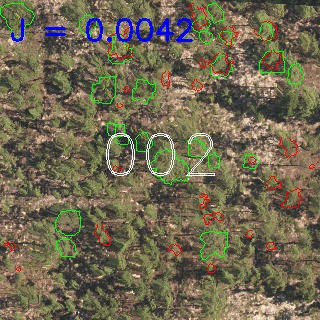
\includegraphics[height=1.8in]{figure/top5_0.jpg} & 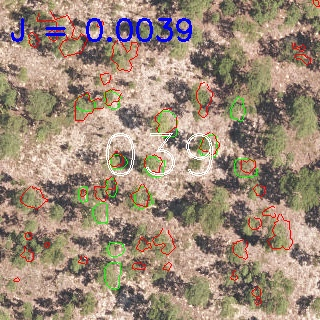
\includegraphics[height=1.8in]{figure/top5_1.jpg} & 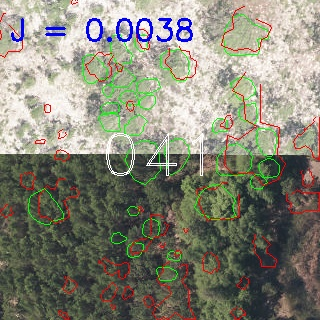
\includegraphics[height=1.8in]{figure/top5_2.jpg} \\
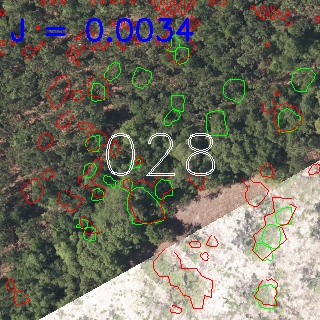
\includegraphics[height=1.8in]{figure/top5_3.jpg} & 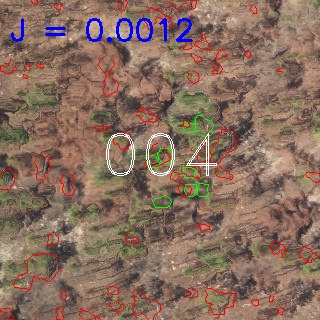
\includegraphics[height=1.8in]{figure/top5_4.jpg} & 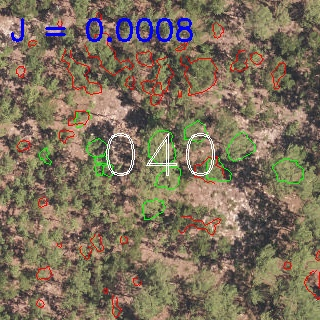
\includegraphics[height=1.8in]{figure/top5_5.jpg} \\
\end{tabular}
\end{table*}

\begin{table*}
\label{tab:top3}
\caption{The worst-6 Delineations}
\center
\begin{tabular}{lll}
\\
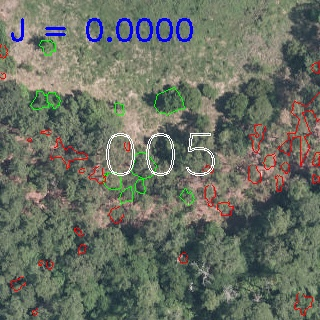
\includegraphics[height=1.8in]{figure/bottom5_0.jpg} & 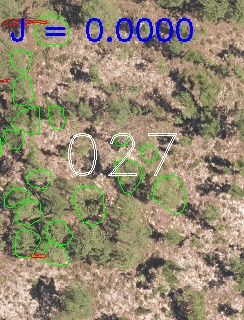
\includegraphics[height=1.8in]{figure/bottom5_1.jpg} & 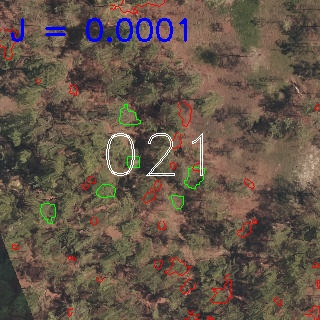
\includegraphics[height=1.8in]{figure/bottom5_2.jpg} \\
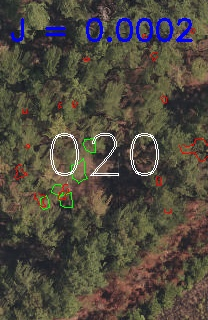
\includegraphics[height=1.8in]{figure/bottom5_3.jpg} & 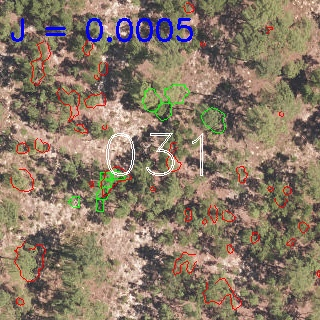
\includegraphics[height=1.8in]{figure/bottom5_4.jpg} & 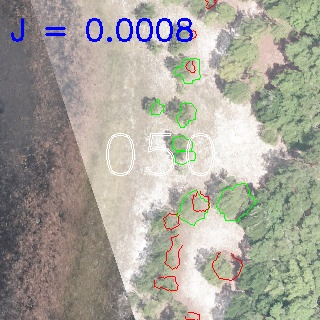
\includegraphics[height=1.8in]{figure/bottom5_5.jpg} \\
\end{tabular}
\end{table*}





\newpage
\section*{\color{blue}{Task 2 - Crown Alignment}}
\subsection*{Plot-Level Crown Alignment Performance}
While the overall alignment performance gives a good measure for effectiveness of a system, it is also useful to analyze how a system perform w.r.t. each testing plot. Being able to locate those badly performed plots help with finding the source of potential shortcomings, which can be used to further improve the system. The plot-level crown alignment performance is shown in the following figure.
\\
\begin{figure}[H]
    \centering
    \def\svgwidth{0.9\columnwidth}
    \input{crown_alignment.pdf_tex}
    % generated in command line: inkscape -D -z --file=image.svg --export-pdf=image.pdf --export-latex
\end{figure}





\newpage
\section*{\color{blue}{Task 3 - Species Classification}}
\subsection*{Overview of Additional Metrics}
In addition to the cross entropy cost and rank-1 accuracy, we also present the following evaluation metrics for further analysis:
\begin{itemize}
\item[] \textbf{Classification Accuracy:} \input{data/t3_accuracy.dat}
\item[] \textbf{Average F1 score:} \input{data/t3_f1.dat}
\item[] \textbf{Average Specificity:} \input{data/t3_specificity.dat}
% \item[] \textbf{Cohen's Kappa:} \input{data/t3_cohens_kappa.dat}
\end{itemize}

\subsection*{Classification Accuracy}
The accuracy of a classifier is defined as the number of true predictions made by the
classifier divided by the total number of predictions. In our evaluation, accuracy
is computed per class and averaged across all classes to give an average accuracy
score. For class $k$, its accuracy is defined as
\begin{equation}
\textrm{Accuracy}_k = \frac{\textrm{TP}_k+\textrm{TN}_k}{\textrm{TP}_k+\textrm{TN}_k+\textrm{FP}_k+\textrm{FN}_k}
\end{equation}
where:
\begin{itemize}
\item $\textrm{TP}_k$ is the \textbf{True Positive} for class $k$, i.e. number of samples of class $k$ that are classified as class $k$.
\item $\textrm{TN}_k$ is the \textbf{True Negative}, i.e. number of samples not belonging to and not classified as class $k$.
\item $\textrm{FP}_k$ is the \textbf{False Positive}, i.e. number of samples not belonging to class $k$ but classified as class $k$.
\item $\textrm{FN}_k$ is the \textbf{False Negative}, i.e. number of samples of class $k$ but classified as not being class $k$.
\end{itemize}
The per-class classification accuracy is shown in Figure~1.
\newpage
\subsection*{Specificity}
Specificity for a class $k$ refers to the number of samples correctly rejected for a class
$k$ in proprtion to the total number of non-class $k$ samples in the data set. This measurement is used to evaluate the efficiency of classifier in ruling out samples as not belonging to a certain class. A higher specificity means that the classifier can
better reject data points not belonging to a class of species. The average specificity score is calculated as arithmetic mean of specificity scores for all classes. The per-class specificity scores are illustrated in Figure~1.


\begin{figure}
\label{fig:d}
\caption{Accuracy and Specificity Scores (Per-Class).}
    \centering
    \def\svgwidth{\columnwidth}
    \input{t2_as.pdf_tex}
    % generated in command line: inkscape -D -z --file=image.svg --export-pdf=image.pdf --export-latex
\end{figure}


\newpage
\subsection*{Precision, Recall, and F1}
Precision is defined as number of true positive samples divided by the total number of samples predicted as positive by the classifier. For class $k$, it is
\begin{equation}
\textrm{Precision}_k = \frac{\textrm{TP}_k}{\textrm{FP}_k+\textrm{TP}_k}.
\end{equation}
Similarly, recall is the ratio of true positive samples that are correctly identified by the classifier. Mathematically, it is defined as
\begin{equation}
\textrm{Recall}_k = \frac{\textrm{TP}_k}{\textrm{FN}_k+\textrm{TP}_k}.
\end{equation}
The per-class F1 score is thus twice of the harmonic mean of precision and recall, and average F1 score is calculated as arithmetic mean of F1 scores for all classes. The per-class precision, recall and f1 are illustrated in Figure~2.
\\\\\\
\begin{figure}[H]
\label{fig:?}
\caption{F1 Score}
    \centering
    \def\svgwidth{\columnwidth}
    \input{t3_f.pdf_tex}
    % generated in command line: inkscape -D -z --file=image.svg --export-pdf=image.pdf --export-latex
\end{figure}

\begin{figure}[H]
\label{fig:?}
\caption{Precision}
    \centering
    \def\svgwidth{\columnwidth}
    \input{t3_p.pdf_tex}
    % generated in command line: inkscape -D -z --file=image.svg --export-pdf=image.pdf --export-latex
\end{figure}

\begin{figure}[H]
\label{fig:?}
\caption{Recall}
    \centering
    \def\svgwidth{\columnwidth}
    \input{t3_r.pdf_tex}
    % generated in command line: inkscape -D -z --file=image.svg --export-pdf=image.pdf --export-latex
\end{figure}

\newpage
\subsection*{Confusion Matrix}
Finally, we attach the classification confusion matrix where element $(i,j)$ is the sum of probabilities for testing samples from class $i$ predicted as class $j$.
\\\\
\input{data/confusion_matrix.dat}
\end{document}
